\documentclass{article}

\usepackage{graphicx}
\usepackage{tikz}
\usepackage{tikzsymbols}
\usetikzlibrary{calc,patterns,shapes.geometric}
\pagestyle{empty}
\usepackage[margin=0pt]{geometry}
\geometry{papersize={14in,12in}}

\def\centerarc[#1](#2)(#3:#4:#5){\draw[#1] ($(#2)+({#5*cos(#3)},{#5*sin(#3)})$) arc (#3:#4:#5);}

\begin{document}
	\begin{figure}
		\centering
		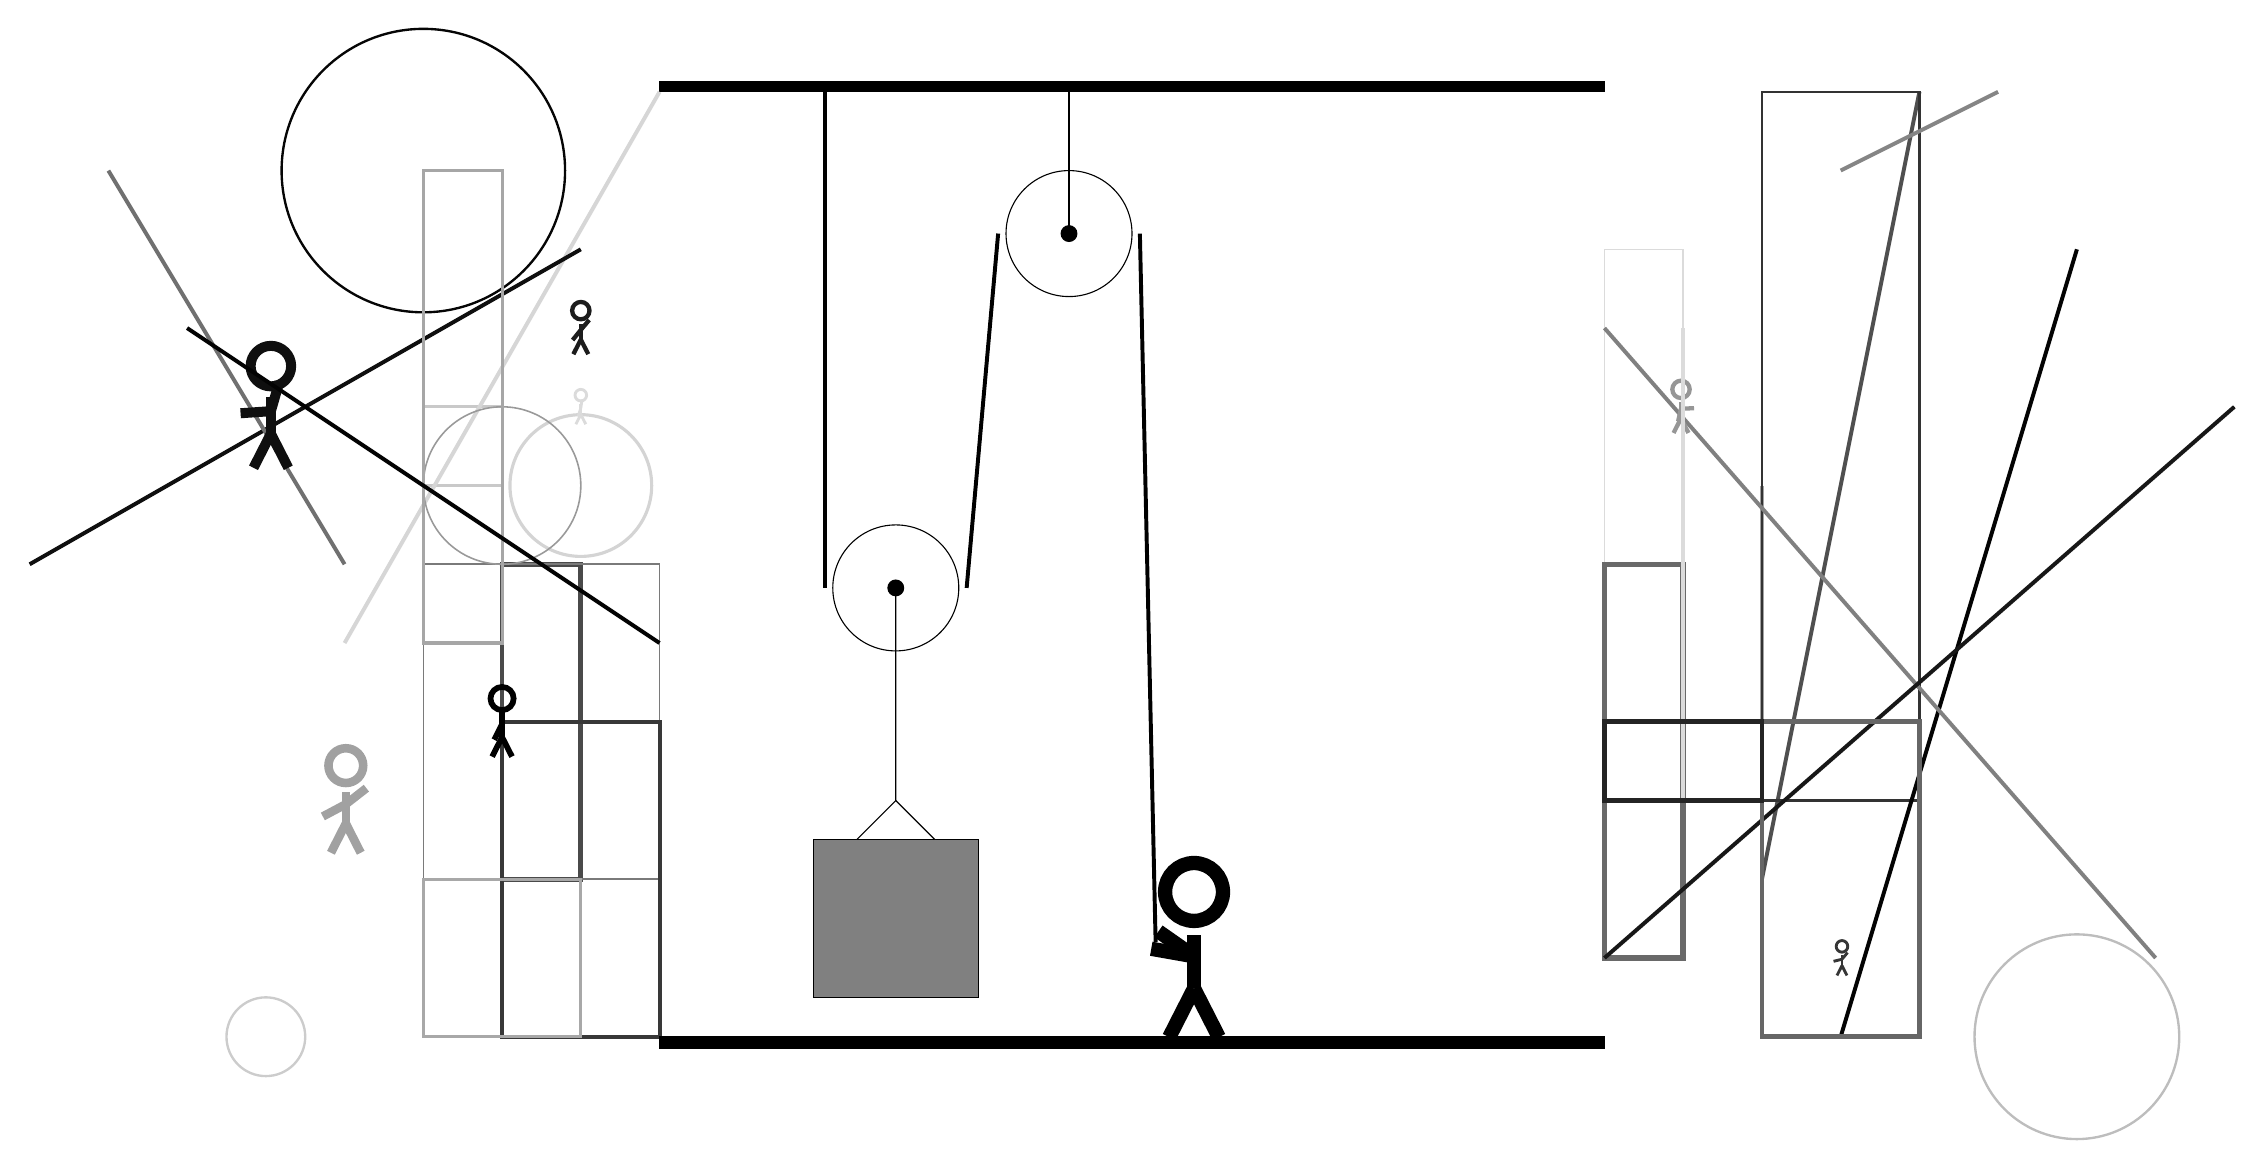
\begin{tikzpicture}
			%%%%% START %%%%%
			
			\draw[fill=black] (-2, 9) rectangle (10, 9.125);
			
			\draw (3.2, 7.2) circle (0.8);
			\draw[fill=black] (3.2, 7.2) circle (0.1);
			\draw[thick] (3.2, 7.2) -- (3.2, 9);
			
			\draw (1, 2.7) circle (0.8);
			\draw[fill=black] (1, 2.7) circle (0.1);
			
			\draw (1, 2.7) -- (1, 0) -- (0.5, -0.5);
			\draw (1, 0) -- (1.5, -0.5);
			\draw[fill=black!50] (-0.05, -0.5) rectangle (2.05, -2.5);
			
			\draw[line width=0.5mm] (0.1, 9) -- (0.1, 2.7);
			\centerarc[line width=0.5mm](1, 2.7)(180:360:0.9);
			\draw[line width=0.5mm](1.9, 2.7) -- (2.3, 7.2);
			\centerarc[line width=0.5mm](3.2, 7.2)(0:180:0.9);
			\draw[line width=0.5mm](4.1, 7.2) -- (4.3, -1.8);
			
			\node at (4.7, -1.9) {\Strichmaxerl[10][-35][170]};
			
			\draw[line width=0.6mm, color=black!71] (-3, 3) rectangle (-4, -1);
			
			\draw [line width=0.4mm, color=black!17](-3, 4) circle (0.9);
			\draw[line width=0.2mm, color=black!14] (10, 7) rectangle (11, 3);
			\draw[line width=0.7mm, color=black!59] (10, 3) rectangle (11, -2);
			\draw[line width=0.2mm, color=black!52] (-2, -1) rectangle (-5, 3);
			\node[line width=0.7mm, color=black!37] at (-6, 0) {\Strichmaxerl[6][28][38]};
			
			\draw [line width=0.3mm, color=black!98](-5, 8) circle (1.8);
			
			\draw[line width=0.5mm, color=black!78] (-4, 1) rectangle (-2, -3);
			\node[line width=0.2mm, color=black!79] at (13, -2) {\Strichmaxerl[2][14][50]};
			
			\draw[line width=0.4mm, color=black!34] (-3, -1) rectangle (-5, -3);
			\draw[line width=0.4mm, color=black!21] (-4, 4) rectangle (-5, 5);
			\draw[line width=0.5mm, color=black!69](14, 9) -- (12, -1);
			\draw[line width=0.5mm, color=black!36](12, -2) -- (12, 4);
			
			\draw[line width=0.3mm, color=black!80] (12, 9) rectangle (14, 0);
			\draw[line width=0.5mm, color=black!48](13, 8) -- (15, 9);
			\draw [line width=0.3mm, color=black!26](16, -3) circle (1.3);
			
			\draw[line width=0.5mm, color=black!16](-6, 2) -- (-2, 9);
			\draw[line width=0.5mm, color=black!94](-3, 7) -- (-10, 3);
			\draw [line width=0.2mm, color=black!40](-4, 4) circle (1.0);
			
			\draw[line width=0.5mm, color=black!56](-6, 3) -- (-9, 8);
			\node[line width=0.4mm, color=black!94] at (-7, 5) {\Strichmaxerl[7][4][74]};
			\draw[line width=0.5mm, color=black!99](13, -3) -- (16, 7);
			\node[line width=0.2mm, color=black!89] at (-3, 6) {\Strichmaxerl[3][51][50]};
			\draw[line width=0.5mm, color=black!50](10, 6) -- (17, -2);
			\draw[line width=0.5mm, color=black!91](10, -2) -- (18, 5);
			
			\node[line width=0.2mm, color=black!100] at (-4, 1) {\Strichmaxerl[4][63][90]};
			\draw [line width=0.3mm, color=black!20](-7, -3) circle (0.5);
			\node[line width=0.4mm, color=black!41] at (11, 5) {\Strichmaxerl[3][77][2]};
			
			\draw[line width=0.7mm, color=black!50] (-4, 8) rectangle (-4, 8);
			\draw[line width=0.5mm, color=black!14](11, 0) -- (11, 6);
			\node[line width=0.7mm, color=black!14] at (-3, 5) {\Strichmaxerl[2][72][82]};
			
			\draw[line width=0.4mm, color=black!35] (-4, 2) rectangle (-5, 8);
			\draw[line width=0.6mm, color=black!60] (12, 1) rectangle (14, -3);
			
			\draw[line width=0.6mm, color=black!86] (12, 0) rectangle (10, 1);
			\draw[line width=0.5mm, color=black!99](-2, 2) -- (-8, 6);
			
			\draw[fill=black] (-2, -3) rectangle (10, -3.15);
			
			%%%%% END %%%%%
		\end{tikzpicture}
	\end{figure}	
\end{document}